\documentclass[11pt, a4paper, titlepage]{article}

% Set document dimensions
\usepackage[paper=a4paper,top=2cm,left=2.5cm,right=2.5cm,bottom=2cm, includefoot]{geometry}
\usepackage{float}
\usepackage[final]{pdfpages} % inludesvg

% Czech fonts
\usepackage[T1]{fontenc}
\usepackage[utf8]{inputenc}
\usepackage[czech]{babel}
\usepackage{fancyhdr}


\usepackage{background}
\backgroundsetup{contents={}}
\setlength{\headheight}{3em} 
\newcommand{\subsectionbreak}{\clearpage}

\begin{document}

	\begin{titlepage}
    % \newgeometry{top=1in,top=2cm,left=2cm,right=2cm,bottom=2cm}

    \centering

    {\fontsize{20pt}{15pt}\bfseries
    VYSOKÉ UČENÍ TECHNICKÉ V~BRNĚ\\
    \vspace{8pt}
    Fakulta informačních technologií
    }


    
\includegraphics[scale=0.7]{./assets/fit-logo.pdf}

    \vspace{22pt}

    {\Large Projekt do předmětu PIS\\}
    \vspace{4pt}
    {\LARGE \bfseries Návrh IS - Knihovna 1 \\}
    {\Large \bfseries Zadádní a návrh převzato z projektu AIS\\}
    \vspace{90pt}
    {\Large \bfseries Tým itsokay\\}
    \vspace{90pt}
    {\Large \today}

    \vspace{90pt}
    {\Large \bfseries Autoři\\}
    \vspace{12pt}

    \begin{tabular}{ l c r }
        Tamaškovič Marek, Bc. (vedoucí týmu)& \texttt{xtamas01} \\
        Kužela Michal, Bc. & \texttt{xkuzel06} \\
        Lakatos Attila, Bc. &\texttt{xlakat01} \\
        Ormoš Michal, Bc. & \texttt{xormos00} \\
    \end{tabular}\\

\end{titlepage}

	\pagestyle{fancy}
	\rhead{
\includegraphics[height=3em]{./assets/bookcase.png}}
	\lfoot{\emph{VUT FIT - PIS}}
	\rfoot{\emph{Tým itsokay}}

	\begin{center}
		\section*{Prvotní analýza a plán projektu}
	\end{center}

	\noindent Následující část dokumentu představuje neformální specifikaci požadavků formou
	strukturovaného textu, prvotní analýzu požadavků včetně UML diagramu případu užití a plán
	projektu s třemi navrženými iteracemi.

	\section*{Neformální specifikace}

	Centrální knihovna ve městě Kocourkov potřebuje pro organizaci své práce, která sestává ze 		správy informací o titulech, čtenářích a jejich pohledávkách nový informační systém, který by
	umožňoval mít všechny údaje pod kontrolou na jednom místě a přehledně zpracované, lépe 	
	vyhovoval současnému stavu fugování knihovny a reflektoval moderní trendy ve vývoji
	informačních systémů.

	Knihovna, která je zadavatelem tohoto projektu sídlí ve městě Kocourkov, a je krajskou 
	knihovnou pro kraj Nadkocourkov. Knihovna poskytuje pro své klienty rozsáhlé spektrum titulů v
	podobě tištěných knih a časopisů. Skládá se ze tří oddělení (pro děti, pro dospělé a oddělení
	odborné literatury). V knihovně pracuje několik zaměstnanců (v řádu jednotlivců), kteří si
	vedou podrobné záznamy o registrovaných čtenářích. V knihovně je také několik zaměstnanců, kteří
	byli jmenováni vedoucími (též administrátory) knihovny. 

	Systém by měl poskytovat informace o stavu jednotlivých titulů v knihovně, o aktuálním umístění 	daného titulu a umožňovat také provést rezervaci tohoto titulu čtenářem. Systém by měl také 
	hlídat maximalní dobu, po kterou uživatel může titul držet a v případě překročení čtenáři 
	udělit pokutu.

	Systém bude implementován jako webová aplikace komunikující s databázovým serverem, který bude
	sloužit jako perzistentní úložiště dat. Od systému se očekává reflektování současných trendů ve
	vývoji informačních systémů, intuitivní a jednotné grafické uživatelské rozhraní a přístupnost
	pro starší uživatele.

	\subsection*{Uživatelé systému}

	Systém by měl umožňovat detailní správu uživatelů. V knihovně se vyskytují 4 skupiny 
	lidí, které reprezentují 4 skupiny uživatelů.

	\begin{enumerate}
		\item Administrátor
		\item Pracovník knihovny
		\item Registrovaný čtenář
		\item Neregistrovaný čtenář
	\end{enumerate}

	\textbf{Neregistrovaný čtenář} není klientem knihovny. Má možnost využívat základních služeb 
	knihovny, avšak nesmí si žádnou knihu zapůjčit a odnést domů. Může tedy v systému
	vyhledávat a filtrovat knihy podle různých kritérií. Systém neregistrovanému čtenáři 
	poskytne základní informace o vyhledané knize a navede jej k jejímu snadnému nalezení.

	\textbf{Registrovaný čtenář} V případě zájmu se z neregistrovaného čtenáře může stát
	registrovaný čtenář. Registraci provádí zaměstnanec knihovny. Jsou mu přiděleny přihlašovací
	údaje do systému. Tím dojde k zásadnímu rozšíření jeho pravomocí.
	Stane se klientem knihovny. U registrovaného čtenáře vzniká povinnost platit pravidelný roční
	registrační poplatek. Registrovaný čtenář má navíc pravomoc si vyhledanou knihu výpůjčit a 		odnést domů. V
	v případě, že kniha není k dispozici, si ji může zarezervovat. Počet výpůjčených knih není omezen.
	Toto může omezit případně zaměstnanec knihovny. Čtenář si může knihu za asistence zaměstnance zapůjčit a
	odsnést domů.

	\textbf{Zaměstnanec knihovny} je člověk, který je s knihovnou v pracovním poměru. Jeho náplní
	práce je obsluha a správa jednotlivých čtenářů. Nové čtenáře může do systému registrovat a
	bývalým čtenářům může profily rušit. Při změně údajů může také profily čtenářů upravovat. Na
	žádost čtenáře provádí operaci zapůjčení a vrácení knihy. Do systému má možnost vkládat nové 		knihy, případně staré knihy nebo knihy o které není zájem vyřazovat. Zaměstnanec také může
	vyřizovat pokuty vzniklé zapomenutím vrácení knihy. Každý rok také vybírá registrační poplatky.
	Obsahuje pravomoce registrovaného čtenáře, což mu umožňuje zarezervovat si knihu pod svým
	zaměstnaneckým profilem.

	\textbf{Administrátor} V knihovně pracuje také několik vedoucích (též administrátorů) knihovny.
	Administrátorem může být jmenován libovolný zaměstnanec. Administrátor poté může
	zakládat profily novým zaměstnancům, rušit profily bývalým zaměstnancům, případně upravovat
	profily stávajícím zaměstnancům. Kvůli střídání pracovní doby může být administrátorem stanoven
	jeden nebo více konkrétních zaměstnanců. Role administrátora také obsahuje pravomoce zaměstnance.

	\subsection*{Kniha a její atributy}

	Každá kniha má svůj název a jméno autora, který knihu sepsal. Kniha je jednoznačne
	identifikována za pomocí ISBN. Dále je uveden počet výtisků, které knihovna vlastní. Je uveden
	také název nakladatelství, které knihu vydalo a datum vydání. Jsou uvedeny jazyky, ve kterých
	je kniha dostupná. U knihy je také uveden typ
	vazby a počet stran. Kniha může být volitelně opatřena krátkým popiskem, který přibližuje knihu
	čtenářům. V rámci knihovny je knihovna zařazena v oddělení, pod žánrem, pod číslem konkrétního
	regálu.

	Systém by měl také umožňovat pro snadnější vyhledávání spravovat kategorie, do kterých 
	jsou knihy zařazeny. Kategorie by mělo být možné interaktivně vytvářet a rušit. Pro usnadnění
	vyhledávání je možné knihám přiřadit také tzv. hashtagy, které umožňují čtenářům
	snadnější vyhledávání v katalogu.

	\subsection*{Vypujčky}
	Doba vypujčky je standartně 1 měsíc. Po vypršení této doby dojde k vytvoření pohledávky, kterou
	je třeba uhradit. Registrovaný čtenář má povinnost uhradit takto vzniklou pohledávku zaměstnanci
	knihovny při následující návštěvě a knihu vrátit. V opačném případě u čtenáře zaniká právo na
	vypůjčení další knihy.
	

	\section*{Analýza požadavků}

	V neformální speicifikaci lze tedy identifikovat čtyři skupiny uživatelů systému, přičemž
	přičemž dvě skupiny jsou návštěvníci knihovny a dvě skupiny jsou zaměstnanci. Následující
	tabulka 1 specifikuje pravomoce, které jsou těmto aktrémům přístupné.

	\begin{table}[!h]
		\centering	
		\label{tab:pravomoce}	
		\begin{tabular}{| c | c |}	
		\hline
		\textbf{Aktér} & \textbf{Pravomoce}\\ 
		\hline	


		Neregistrovaný čtenář & 

		\parbox{.45\textwidth}{
		\begin{itemize}
		    \item Vyhledání knihy
		    \item Zobrazení detailních informací o knize
		\end{itemize}} 
		\\

		\hline

		Registrovaný čtenáč & 
		\parbox{.45\textwidth}{\begin{itemize}
		    \item Rezervace knihy
		    \item Zrušení rezervace knihy
		    \item + Vše co neregistrovaný čtenář
		\end{itemize}} 
		\\

		\hline
		
		Zaměstnanec knihovny & 
		\parbox{.45\textwidth}{\begin{itemize}
		    \item Zapůjčení knihy registrovanému čtenáři
		    \item Převzetí knihy od čtenáře a vrácení knihy do knihovny
		    \item Splacení pohledávky
		    \item Přidání knihy
		    \item Odebrání knihy
	            \item Úpravy knihy
		    \item Registrace účtu klienta
		    \item Editace účtu reg. čtenáře
		    \item Smazání účtu reg. čtenáře
	            \item + Vše co registrovaný čtenář
		\end{itemize}} 
		\\

		\hline

		Administrátor & 
		\parbox{.45\textwidth}{\begin{itemize}
		    \item Registrace zaměstnance
		    \item Smazání zaměstnance
		    \item Úpravy zaměstnance
	            \item + Vše co zaměstnanec
		\end{itemize}} 
		\\
		\hline
  		
		\end{tabular}
		\caption{Rozdělení pravomocí jednotlivým aktérům, role uživatelů}
	\end{table}

	\noindent Využití dědičnosti aktérů vyplynulo ze společných požadavků na aktéry v různých
	rolích.

	Pro zamezení duplicičnosti uživatelských profilů je zaměstnanecký a čtenářský profil 
	zaměstnance sloučen v jeden. V případě, že je zaměstnanec zároveň registrovaným čtenářem,
	tak jako čtenář vystupuje pod svým zaměstnaneckým profilem.

	\newpage

	Následující diagram užití přehledně zobrazuje případy užití asociované s výše uvedenými aktéry	
	\footnote{V diagramu jsou pouze případy užití specifické pro daný systém. Nejsou znázorněny
	případy užití související s autentizací a autorizací, které jsou u informačních systémů
	všeobecně známé.}.
	
	\begin{figure}[H]
		
		\centering
		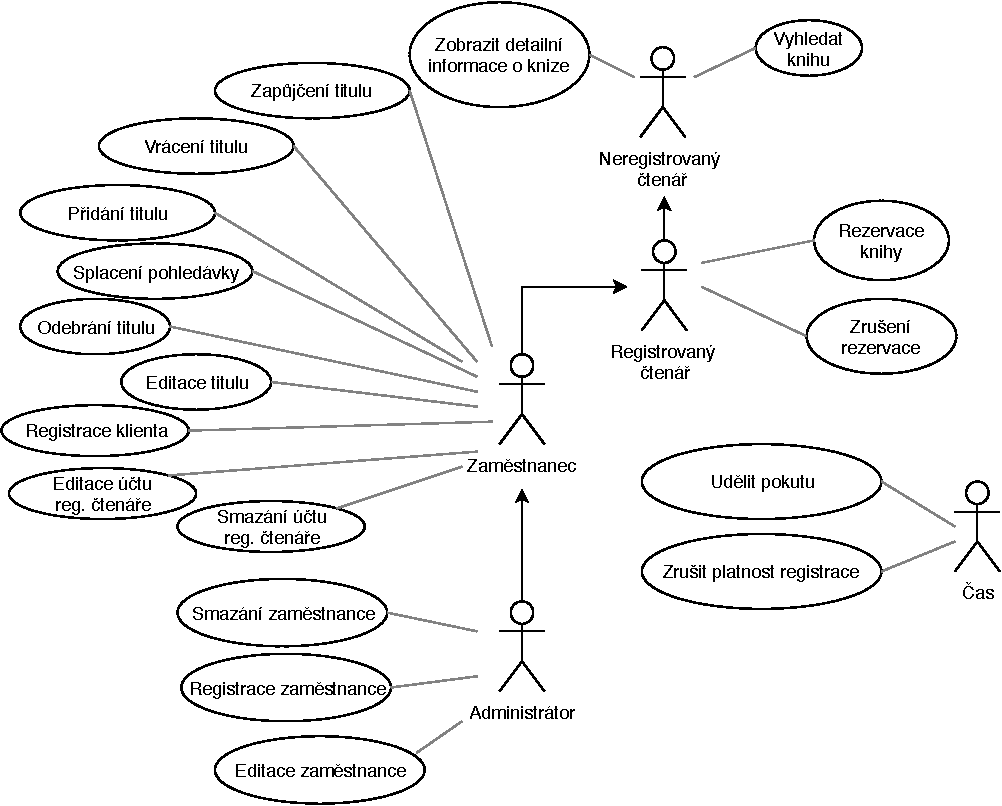
\includegraphics[width=1.0\textwidth, angle=0]{./assets/usecase/full.pdf}
		\caption{UML diagram znázorňující navržený systém a případy užití}

	\end{figure}

	\begin{figure}[H]
		\centering
        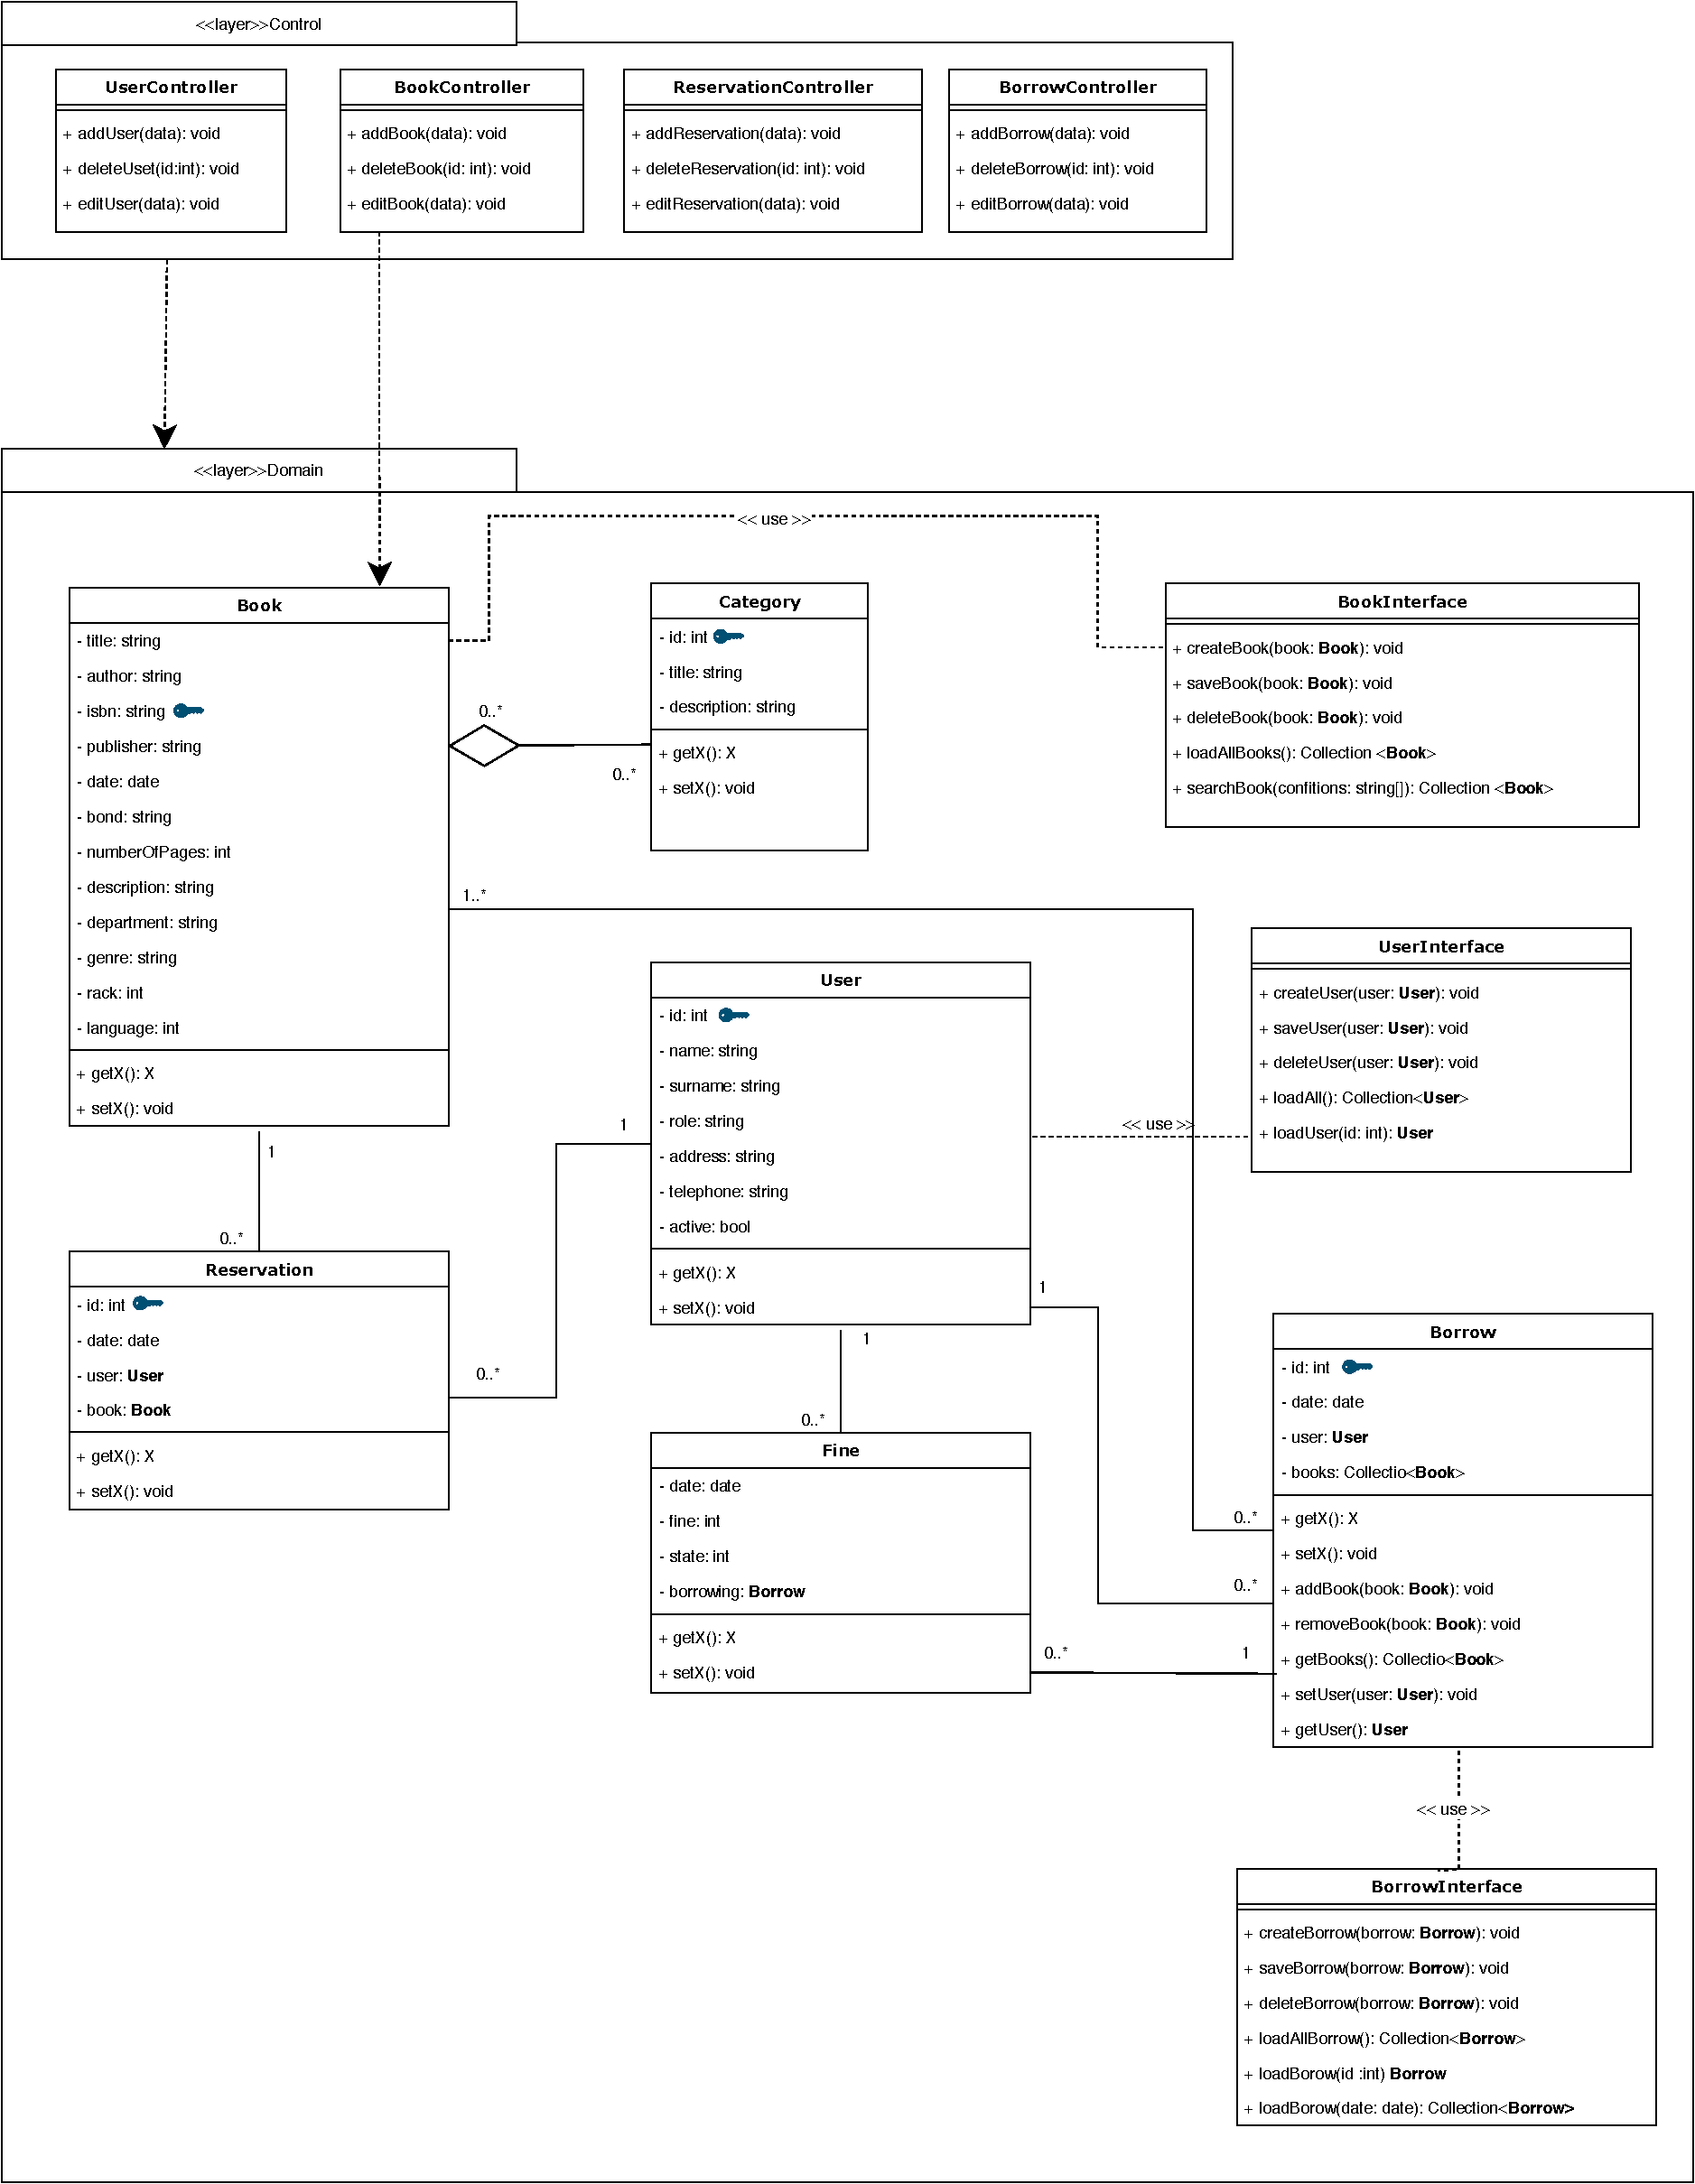
\includegraphics[width=1.0\textwidth]{./assets/classdiagram/KDM.pdf}
		\caption{Návrhový diagram tříd}
	\end{figure}

	\newpage
	\section*{Implementace}
	Pro tenhle projekt sme se rozhodli použít technologie Laravel + Patternfly.
	\begin{itemize}
	    \item Laravel je moderní PHP franework, jehož užití většina tímu dobře zná.
	    \item Patternfly je UI framework, kterej nás nejvíc zaujal z možných frameworku pro účely uživatelského rozhraní.
	\end{itemize}{}


\end{document}
